\documentclass[tikz,border=10pt]{standalone}
% Shared style for all project diagrams
\usepackage{amsmath,amssymb}
\usetikzlibrary{positioning,arrows.meta,calc,fit,decorations.pathreplacing}
\renewcommand{\familydefault}{\sfdefault}
\definecolor{accent}{RGB}{42,120,214}
\definecolor{lblue}{RGB}{234,242,252}
\definecolor{card}{RGB}{247,247,245}
\definecolor{ink}{RGB}{17,17,17}
\definecolor{gray52}{RGB}{82,81,78}
\definecolor{dblue}{RGB}{13,54,107}
\tikzset{
  box/.style={draw=accent, thick, rounded corners=3pt, fill=lblue, align=center,
              minimum height=1.05cm, inner sep=6pt, text=ink},
  plain/.style={draw=gray52!60, thick, rounded corners=3pt, fill=card, align=center,
              minimum height=1.05cm, inner sep=6pt, text=ink},
  ghost/.style={align=center, text=gray52, font=\footnotesize},
  arr/.style={-{Stealth[length=2.6mm]}, very thick, draw=accent},
  garr/.style={-{Stealth[length=2.6mm]}, thick, draw=gray52},
  lbl/.style={font=\footnotesize, text=gray52, align=center},
}

\begin{document}
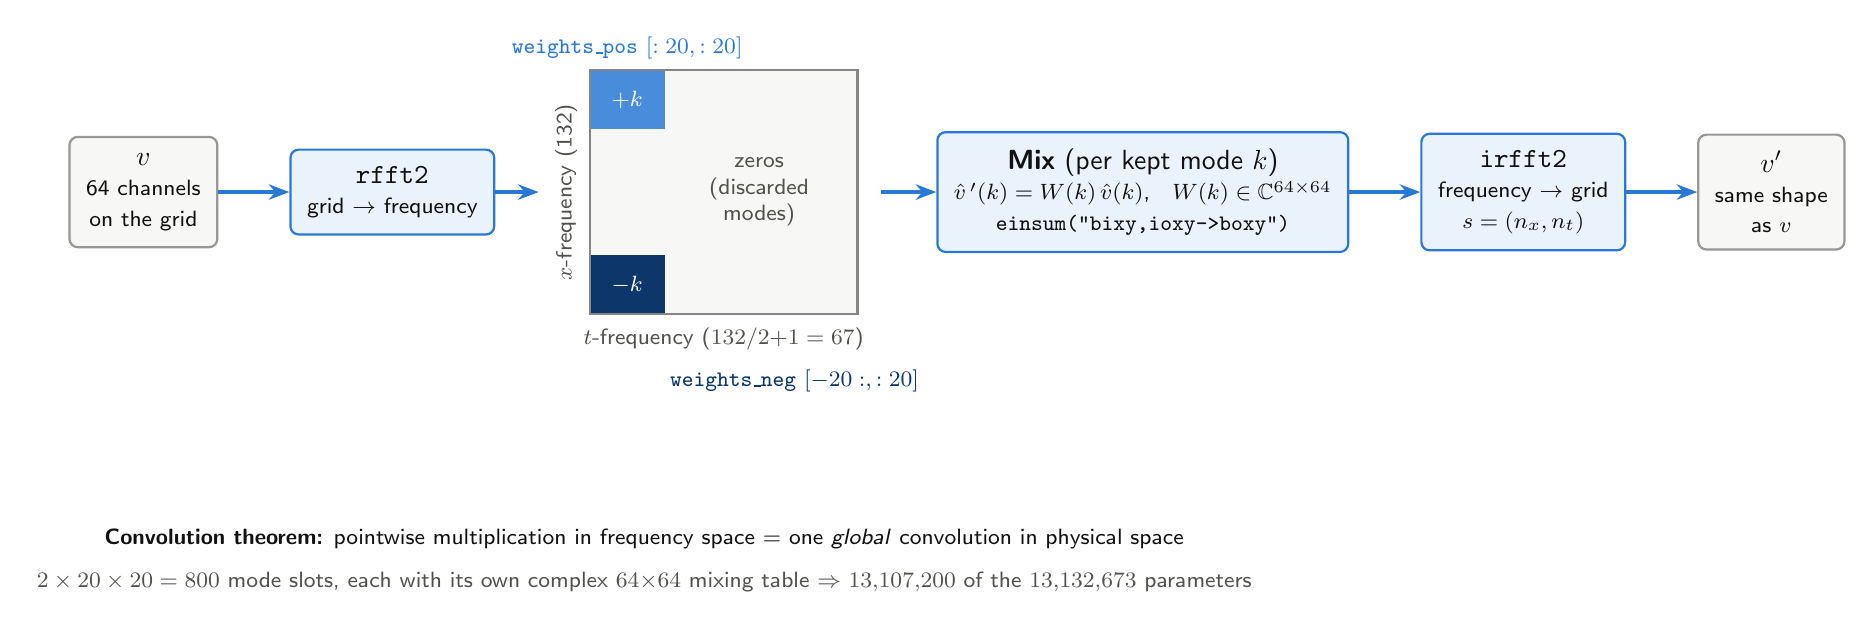
\begin{tikzpicture}[node distance=0.6cm and 0.9cm]
  \node[plain] (vin) {$v$\\[-1pt] {\footnotesize 64 channels}\\[-1pt] {\footnotesize on the grid}};
  \node[box, right=of vin] (fft) {\texttt{rfft2}\\[-1pt] {\footnotesize grid $\to$ frequency}};

  % ---- frequency array picture -------------------------------------
  \begin{scope}[shift={($(fft.east)+(1.2,-1.55)$)}]
    % full array 132 x 67 (x-freq vertical, t-freq horizontal)
    \draw[fill=card, draw=gray52!70, thick] (0,0) rectangle (3.4,3.1);
    % kept blocks (t modes: left edge; x modes: top = +k, bottom = -k)
    \fill[accent!85] (0,2.35) rectangle (0.95,3.1);   % weights_pos  [:20,:20]
    \fill[dblue]     (0,0)    rectangle (0.95,0.75);  % weights_neg  [-20:,:20]
    \draw[gray52!70, thick] (0,0) rectangle (3.4,3.1);
    \node[lbl, text=white] at (0.475,2.72) {$+k$};
    \node[lbl, text=white] at (0.475,0.37) {$-k$};
    \node[lbl] at (2.15,1.55) {zeros\\ (discarded\\ modes)};
    % axes labels
    \node[lbl, rotate=90] at (-0.3,1.55) {$x$-frequency (132)};
    \node[lbl] at (1.7,-0.32) {$t$-frequency ($132/2{+}1 = 67$)};
    \node[lbl, text=accent] at (0.475,3.38) {\texttt{weights\_pos} $[:20,:20]$};
    \node[lbl, text=dblue]  at (2.6,-0.85) {\texttt{weights\_neg} $[-20:,:20]$};
  \end{scope}

  % ---- mix and inverse ----------------------------------------------
  \node[box, right=5.6cm of fft, minimum width=4.4cm] (mix)
    {\textbf{Mix} (per kept mode $k$)\\[-1pt]
     {\footnotesize $\hat v^{\,\prime}(k) = W(k)\,\hat v(k)$, \; $W(k)\in\mathbb{C}^{64\times64}$}\\[-1pt]
     {\footnotesize \texttt{einsum("bixy,ioxy->boxy")}}};
  \node[box, right=of mix] (ifft) {\texttt{irfft2}\\[-1pt] {\footnotesize frequency $\to$ grid}\\[-1pt] {\footnotesize $s=(n_x,n_t)$}};
  \node[plain, right=of ifft] (vout) {$v'$\\[-1pt] {\footnotesize same shape}\\[-1pt] {\footnotesize as $v$}};

  \draw[arr] (vin) -- (fft);
  \draw[arr] (fft.east) -- ++(0.55,0) node[midway, lbl, above=1pt] {} ;
  \draw[arr] ($(fft.east)+(4.9,0)$) -- (mix.west);
  \draw[arr] (mix) -- (ifft);
  \draw[arr] (ifft) -- (vout);

  \node[lbl, below=3.6cm of fft, xshift=3.2cm, text=ink]
    {\textbf{Convolution theorem:} pointwise multiplication in frequency space
     $=$ one \emph{global} convolution in physical space};
  \node[lbl, below=4.15cm of fft, xshift=3.2cm]
    {$2\times20\times20 = 800$ mode slots, each with its own complex $64{\times}64$ mixing table
     $\Rightarrow$ $13{,}107{,}200$ of the $13{,}132{,}673$ parameters};
\end{tikzpicture}
\end{document}
